\bluepage{OpenGL}

\begin{frame}
\frametitle{OpenGL}
  \begin{itemize}
  \item OpenGL Open Graphics Language (Library) 
  \item OpenGL is API for 3D accelerated graphics 
  \item OpenGL is platform independent
  \item OpenGL wrapper ported to most languages
  \item Main goal of OpenGL is to convert scene represented using 3D vectors to 2D rasterized image
  \item OpenGL can be used for arbitrary computation since OpenGL 4.3
  \item OpenGL specification contains description of it's GPU language GLSL
  \end{itemize}
  \begin{figure}[h]
  
\includegraphics[width=5cm,keepaspectratio]{pics/opengl_logo.jpg}
  \end{figure}
\end{frame}

\begin{frame}
\frametitle{OpenGL architecture}
  \begin{itemize}
    \item OpenGL can be viewed as client-server architecture
    \item User application runs on CPU and through OpenGL calls can control GPU
  \end{itemize}
  \begin{figure}[h]
    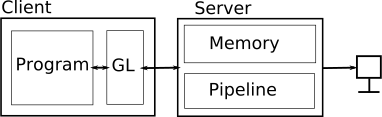
\includegraphics[width=10cm,keepaspectratio]{pics/clientserver.pdf}
  \end{figure}
\end{frame}

\begin{frame}
\frametitle{OpenGL 4.3 pipeline}
  \begin{figure}[h]
  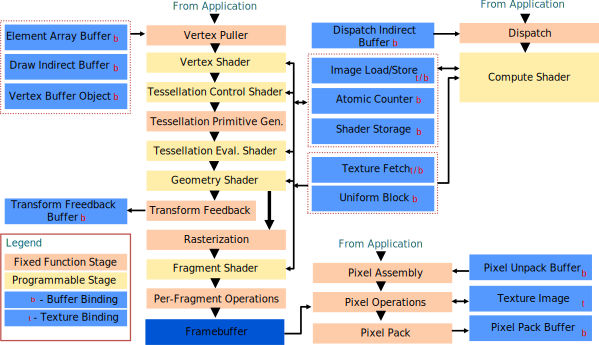
\includegraphics[width=10cm,keepaspectratio]{pics/opengl43_2.pdf}
  \end{figure}
\end{frame}

\begin{frame}[fragile]
\frametitle{Frame Buffer Object (FBO)}
  \begin{itemize}
    \item A scene is, in most cases, rendered into default framebuffer
    \item Since OpenGL 3.3, it is possible to creates custom framebuffers.
    \item Each framebuffer is composed of set of color textures and depth and stencil texture
    \item Framebuffers allows rendering into textures
    \item Textures do not have to store color but they can store other useful information as well (positions, normals, depths, ...)
    \item They can be used as intermediate stages in rendering pipeline
  \end{itemize}
\end{frame}

\begin{frame}[fragile]
\frametitle{FBO example - creation of textures}
  {\scriptsize
  \begin{minted}[frame=lines]{c++}
//reserve texture id
glGenTextures(1,&tColor);

//bind texture to 2D target
glBindTexture(GL_TEXTURE_2D,tColor);

//set filtering
glTexParameteri(GL_TEXTURE_2D,GL_TEXTURE_MAG_FILTER,GL_NEAREST);
glTexParameteri(GL_TEXTURE_2D,GL_TEXTURE_MIN_FILTER,GL_NEAREST);

//allocate memory on GPU and copy data from CPU
glTexImage2D(GL_TEXTURE_2D,0,GL_RGBA,width,height,0,GL_RGBA,
GL_UNSIGNED_BYTE,data);
  \end{minted}
  }
\end{frame}

\begin{frame}[fragile]
\frametitle{FBO example - initialization}
  {\scriptsize
  \begin{minted}[frame=lines]{c++}
//reserver framebuffer id
glGenFramebuffers(1,&FBO);
//bind framebuffer
glBindFramebuffer(GL_FRAMEBUFFER,FBO);

//set framebuffer attachments
glFramebufferTexture2D(GL_FRAMEBUFFER,GL_COLOR_ATTACHMENT0,
  GL_TEXTURE_2D,tColor,0);//attach color texture
glFramebufferTexture2D(GL_FRAMEBUFFER,GL_COLOR_ATTACHMENT1,
  GL_TEXTURE_2D,tNormal,0);//attach normal texture

GLenum H[]={
  GL_COLOR_ATTACHMENT0,//layout(location=0)out vec4 fragColor;
  GL_COLOR_ATTACHMENT1//layout(location=1)out vec3 fragNormal;
};
glDrawBuffers(2,H);//set set of targets
glBindFramebuffer(GL_FRAMEBUFFER,0);//unbind framebuffer
  \end{minted}
  }
\end{frame}

\begin{frame}[fragile]
\frametitle{FBO example - drawing}
  {\scriptsize
  \begin{minted}[frame=lines]{c++}
//activate framebuffer
glBindFramebuffer(GL_FRAMEBUFFER,FBO);

//...

//draw some geometry
glDrawArrays(GL_TRIANGLE_STRIP,0,4);

//...

//deactivate framebuffer
glBindFramebuffer(GL_FRAMEBUFFER,0);
  \end{minted}
  }
\end{frame}

\begin{frame}[fragile]
\frametitle{FBO example - blitting}
  Data from one framebuffer can be transfered into another framebuffer using blit operation.
  {\scriptsize
  \begin{minted}[frame=lines]{c++}
//activate source framebuffer
glBindFramebuffer(GL_READ_FRAMEBUFFER,FBO0);

//active destination framebuffer
glBindFramebuffer(GL_DRAW_FRAMEBUFFER,FBO1);

//copy color buffers
glBlitFramebuffer(
  srcX0,srcY0,
  srcX2,srcY1,
  dstX0,dstY0,
  dstX1,dstY1,
  GL_COLOR_BUFFER_BIT,
  GL_NEAREST);

//deactivate framebuffers
glBindFramebuffer(GL_READ_FRAMEBUFFER,0);
glBindFramebuffer(GL_DRAW_FRAMEBUFFER,0);
  \end{minted}
  }
\end{frame}


